
\section{Signal Model}

This analysis studies the simplified model shown in Figure \ref{fig:feyn}, targeting primarily the decays via Higgs boson.
These are models of \gls{ggm} \cite{Meade:2008wd,Cheung:2007es,Dine:1981gu,AlvarezGaume:1981wy,Nappi:1982hm} 
(already discussed in Section \ref{sec:susybreaking})
or \gls{gmsb} \cite{Dimopoulos:1996vz,Matchev:1999ft} where 
the lightest neutralino is the \gls{nlsp}, that decays promptly to the gravitino ($\gravino$), which is the \gls{lsp}, and 
a \gls{sm} boson. 

\begin{figure}[htbp]
	\centering
	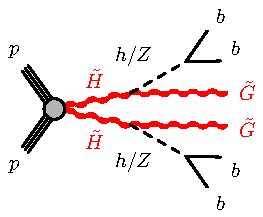
\includegraphics[width=0.35\textwidth]{figures/ewk_prod/varie/N1N1-hhGG-bbbb_Z}
	\caption{Diagram for the simplified model considered in the analysis. The primary interpretation of the analysis is the decay via Higgs bosons, but decays via varied branching ratios to $Z$ bosons are also studied. The production of the \hino\ occurs
via mass-degenerate pairs of charginos or neutralinos, which decay to the \ninoone\ and immeasurably low momentum particles.} 
	\label{fig:feyn}
\end{figure}

As discussed in Section \ref{sec:theo:mssm} \gls{susy} predicts five Higgs bosons. 
Their superpartners (higgsinos) mix with the superpartners of the electroweak gauge bosons to form charginos and neutralinos.

In models where the the lightest neutralinos and charginos are dominated by the higgsino component, the four lightest charginos 
and neutralinos are nearly degenerate \cite{Papucci:2011wy,Barbieri:2009ev,Han:2014kaa} and ordered as: $m_{\tilde\chi^0_1}~<~m_{\tilde\chi^\pm_1}~<~m_{\tilde\chi^0_2}$.
These models are particularly interesting because they arise in the limit where $|\mu| < |M_1|, |M_2$|, which is the same limit 
that minimizes the fine tuning problem in the Higgs sector of the \gls{mssm}.

In the case of a higgsino-like neutralino, the direct production of a \ninoone\ninoone\ pair is suppressed, and the production cross section is dominated by 
\ninoone\ninotwo, \ninoone\chinoonepm, \ninotwo\chinoonepm, and \chinoonep\chinoonem production.
The \ninotwo and \chinoonepm then decay to the \ninoone and soft particles that can not be detected (originating from the 
decay of off-shell W and Z bosons), therefore all of these production processes give practically the same final state as 
\ninoone\ninoone\  pair production. 

Since in this chapter we consider only the case where the lightest neutralino is dominated by the higgsino component,
we will use interchangeably the notation \ninoone or \hino to indicate it.  
We consider only the case where the lifetime of the \hino is very short and it decays promptly to a Higgs boson or a Z boson and the \gravino;
this is the case when the mass of the mediators of \gls{susy} breaking is relatively small (smaller than $\approx 10^7$ GeV), 
while for higher mediator masses the \gls{nlsp} acquires a finite lifetime, and can pass through the full detector without decaying. 


\subsection{Signal cross section}

The signal cross section is computed for the pure higgsino case, at \gls{nlo} plus \gls{nll} precision, assuming that
\ninoone, \ninotwo and \chinoonepm are degenarate and that all the other \gls{susy} particles decouple \cite{Fuks:2012qx,Fuks:2013vua}.
The nominal cross section and its uncertainty are taken from an envelope of two cross section predictions using different \gls{pdf} sets, 
and it is 3830 $\pm$ 160 fb at $\mhino = 150$ GeV, while it decreases to 1.8 $\pm$ 0.2 fb at $\mhino = 900$ GeV. 

\subsection{Higgsino decay modes}

This search is optimized to target cases where both \hino decay promptly to a Higgs boson and a gravitino. 



%\section{Previous Limits}

